\documentclass[18pt, oneside]{article}   	
\usepackage{geometry}                		
\geometry{letterpaper}   
\usepackage[utf8]{inputenc}
\usepackage{amsmath}                		 
%\geometry{landscape}                		
%\usepackage[parfill]{parskip}    		
\usepackage{graphicx}				
\usepackage{tikz}										
\usetikzlibrary{shapes.misc}
\usetikzlibrary{backgrounds}
\tikzset{cross/.style={cross out, draw=black, minimum size=2*(#1-\pgflinewidth), inner sep=0pt, outer sep=0pt},
%default radius will be 1pt. 
cross/.default={1pt}}

\usepackage{amssymb}
\setlength{\parindent}{0pt}
\title{HW4-Lecture notes}
\author{Jody Shu, Yiping Lu, Jashaina Thomas}
%\date{}							

\begin{document}
\maketitle
%\section{}
%\subsection{}
\begin{Large}
\textbf{Q}: What if the data is not linear separable?

\vspace*{1cm}\hspace{6cm}%
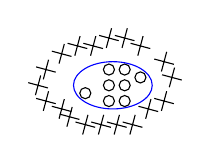
\begin{tikzpicture}[]



\draw (7,5) circle (2pt);
\draw (7,5.2) circle (2pt);
\draw (7,5.4) circle (2pt);
\draw (6.8,5) circle (2pt);
\draw (6.8,5.2) circle (2pt);
\draw (6.8,5.4) circle (2pt);
\draw (6.5,5.1) circle (2pt);
\draw (7.2,5.3) circle (2pt);

\draw (7.5,5) node[cross=3pt,rotate=30] {};
\draw (7.6,5.3) node[cross=3pt,rotate=30] {};
\draw (7.5,5.5) node[cross=3pt,rotate=30] {};

\draw (7.3,4.9) node[cross=3pt,rotate=30] {};
\draw (7.1,4.7) node[cross=3pt,rotate=30] {};
\draw (6.9,4.7) node[cross=3pt,rotate=30] {};
\draw (6.7,4.7) node[cross=3pt,rotate=30] {};
\draw (6.5,4.7) node[cross=3pt,rotate=30] {};
\draw (6.3,4.8) node[cross=3pt,rotate=30] {};
\draw (6.2,4.9) node[cross=3pt,rotate=30] {};
\draw (6.,5) node[cross=3pt,rotate=30] {};
\draw (5.9,5.2) node[cross=3pt,rotate=30] {};
\draw (6.,5.4) node[cross=3pt,rotate=30] {};
\draw (6.2,5.6) node[cross=3pt,rotate=30] {};
\draw (6.4,5.7) node[cross=3pt,rotate=30] {};
\draw (6.6,5.7) node[cross=3pt,rotate=30] {};
\draw (6.8,5.8) node[cross=3pt,rotate=30] {};
\draw (7,5.8) node[cross=3pt,rotate=30] {};
\draw (7.2,5.7) node[cross=3pt,rotate=30] {};
\draw[ color=blue] (6.85,5.2) ellipse (0.5 and .3);
\end{tikzpicture}
\\
\textbf{Ans}: Use Kernel method.



\section{Kernel methods}
\subsection{Introduction}
Kernel methods are a class of algorithms for pattern analysis, whose best known member is the support vector machine (SVM). The general task of pattern analysis is to find and study general types of relations in datasets. Kernel methods owe their name to the use of kernel functions, which enable them to operate in a high-dimensional, implicit feature space without ever computing the coordinates of the data in that space, but rather by simply computing the inner products between the images of all pairs of data in the feature space. This operation is often computationally cheaper than the explicit computation of the coordinates. This approach is called the "kernel trick". Kernel functions have been introduced for sequence data, graphs, text, images, as well as vectors.
\subsection{Kernel matrix}
\begin{equation}
\Phi(\vec{x})^\top = 
\begin{bmatrix}
\Phi(x_{1})^\top\\
\Phi(x_{2})^\top\\
\vdots
\Phi(x_{n})^\top
\end{bmatrix}
\end{equation}

\begin{equation}
\begin{bmatrix}
\Phi(x_{1})^\top\\
\Phi(x_{2})^\top\\
\vdots
\Phi(x_{n})^\top
\end{bmatrix}
\begin{bmatrix}
\Phi(x_{1}) & \Phi(x_{2}) & \cdots & \Phi(x_{n})
\end{bmatrix}=
\begin{bmatrix}
\Phi(x_{1})^\top\Phi(x_{1}) & \Phi(x_{1})^\top\Phi(x_{2}) & \cdots \\
\Phi(x_{2})^\top\Phi(x_{1})\\
\vdots
\end{bmatrix}
\end{equation}
Property: This matrix is positive semidefinite! $\forall \vec{u}$, 
\begin{equation}
\vec{u}^\top\Phi(x)^\top\Phi(x)\vec{u} = (\Phi(x)\vec{u})^\top(\Phi(x)\vec{u}) = \|\Phi(x)\vec{u}\|^2 \geq 0
\end{equation}
Example: $(x^{i}, y^{i})$
\begin{equation}
K(x,y) = (2<x,y> + 5)^2
\end{equation}
\end{Large}
\end{document}




